\chapter{A survey of Cognitive Architectures}
\label{The_nature_of_cognition}

The quest to understand the working of the human mind has spanned
many centuries starting with Plato when he asked, as in the words of
Noam Chomsky citing Bertrand Russell, ``{\bf How is it that human beings,
whose contacts with the world are brief, personal and limited, are
nevertheless able to know as much as they do?}'' \cite{Bogdan:1993aa}


Cognitive science brings together the varied disciplines of
psychology, neuroscience, computer science, linguistics and philosophy
in an attempt to answer the above question, using information
processing as a means to emulate the human mind. Psychology,
especially cognitive psychology, contributes theories on cognitive
capacities, information processing capabilities of , and so forth.
Perhaps most importantly, it theorizes about the overall picture of
the human mind. Neuroscience, the study of the brain and nervous
system, provides a frame of reference against which theories developed
in cognitive science can be validated since it deals with the brain at
the lowest level.
% 
% Secondly, it provides knowledge for developing an alternative
% architecture of the mind. -- I was reffering to the connectionist
% architectures.
%
Computer science contributes knowledge representation, which is used
to develop theories to represent the way knowledge is stored,
artificial intelligence, which is used to analyse and create methods
for problem solving, and the theory of computation, which is used as a
means to understand foundational limits on cognition as
information processing.

The objective of this chapter is three-fold.  Firstly it aims to
provide a very brief introduction to the human cognitive architecture
from both the cognitivist and emergent
\cite{DBLP:journals/tec/VernonMS07} perspectives.  Secondly it
discusses cognitive architecture in general.  Finally it goes on to
compare some currently and widely used cognitive architectures.

\section{The nature of cognition}
\label{nature_Of_Cognition}
Any attempt to deal with the architecture of cognition has to answer
the following questions.

\begin{itemize}
\item \emph{What is knowledge and how can it be categorized?}  Since the aim
  of cognitive science is to understand the working of the human mind
  it is essential the nature of knowledge is understood because human
  beings function by processing information. Therefore it is
  imperative that we understand what knowledge is and the different
  forms of knowledge that are available.

  Although the nature of knowledge has been studied over many
  millennia we are still not certain of its characteristics. Here I
  will briefly describe what Brachman and Levesque in
  \cite{brachman-levesque:2004a} have to say about the nature of knowledge.
  They describe as one perspective of knowledge as a function that
  maps a knower to a proposition. A proposition is a statement that
  determines the truth value of the belief of the knower. But they
  also acknowledge that not all knowledge is of this form, for example

\item \emph{How is knowledge acquired, represented and utilized?} When
  solving problems the human mind has the ability to retrieve and
  apply previously stored knowledge to the problem; for example,
  consider solving a calculus based integration problem.  We are able
  to retrieve standard representations of the forms of equations and
  apply them to the problem to simplify it and solve it.   Issues
    of knowledge retrieval and application are central to
  understanding cognition.

\item How do various processes act on this knowledge and how do they
  achieve the effect they intend to achieve?  These two areas are
  significant because of their relationship to the techniques of
  deduction and inference that we use to solve problems on an everyday
  basis, inferences as simple and routine as when we diagnose a faulty
  light, or the more complex techniques we use when solving a
  crossword puzzle.

\item How can these processes and structures be manifested in the real
  world? \textsc{Waiting for prof response}
\end{itemize}


These questions provide us with a very general framework of the
results to be provided by cognitive
science. Newell~\cite{,Newell1980135} describes the study of the
working of the mind as a problem of satisfying the ``Conjunction of
constraints on the nature of mind like systems.'' He describes the
characteristics of what is to be expected of any theory that claims to
propose a model of human cognition. Newell mentions that this list is
not comprehensive, but in the view of Anderson and Lebiere~\cite{} it
can used to provide a broad framework against which all theories that
claim to explain the human mind can be tested.
 
These criteria, listed below, have been discussed in the
literature~\cite{CambridgeJournals:207162,Newell:1990aa}. The purpose
of listing these criteria below is to explain as to what the study of
the mind would require.

\begin{itemize} 


\item Behave flexibly as a function of the environment: At first
glance this statement may seem frivolous, as it seems to imply that
human cognition functions in a haphazard manner. But Newell did make it clear
that he was referring to the view that a cognitive system can be
viewed as an instance of a universal computer, specifically a turing
machine, despite its occasional failings and lack of infinite
memory. He further explains that this view does not indicate the
inablity to perform special operations, for example, vision. He
explains that like computers with special processing units the
cognitive system can be made up of special purpose systems that
specialize in a certain task. As an example consider the example of
chemist they are able to perform congnitive tasks that are relates to
their field and they are also able to drive their car. 


\item Operate in real time: A system that models cognition should be
able to explain the reason as to how we are able to perform cognitive
tasks at the speed humans do. This criteria is important because if a
system is not able to explain it could lead us to wrong assumptions
about how humans think.


\item Exhibit rational adapative behaviour: It must be able to explain
this because humans perform computations and those computations, as in the words of
Newell\cite{Newell:1990aa}, are for ``the service of goals and
rationally related to obtaining things that let the organism survive
and propagate.''

\item Display dynamic behaviour: Humans operate in an
environment that is ever changing. They draw in this
information from their environment and act on it appropriately. For
example, if you are driving a car and at that moment a deer decides
to sprint in front of the car, you would hit the brakes. 


\item Integrate diverse knowledge: Humans acquire knowledge from
diverse sources and are able to integrate them. For example consider a
computer programmer working in the banking industry. He can go to
school to obtain knowledge of the working of the finance industry. He
can use this knowledge along with his knowledge of computers science
to write programs for the industry. Here we see that our fictitious
programmer integrating knowledge, unlike expert systems where
knowledge is vertical and cannot be integrated as easily.

\item Exhibits a sense of consciousness: Newell could not point out to
  the direct relation between consciousness and human cognition but he
  did mention it as one of the criteria in his tests of human
  cognition. One interpretation of
  this~\cite{CambridgeJournals:207162} is that Newell was asking us to
  pick out criteria for this test and the authors of that paper point
  towards using sections from \cite{Cohen:1996aa}

\item Learning from the environment: This point should be self
evident, we gain new knowledge from the world around us. But then
the type of learning itself should be based on whether it can learn based on
semantic memory, skill, priming and conditioning.

\item Arise through evolution: It is understood that the algorithms we
use today are those that have arisen naturally over a period of time,
hence any cognitive architecture should be able to learn and improve
the algorithms through an process of constant improvement.

\item Use of Natural language: Any theory that claims to decipher human
cognition must be able to explain as to how we are able to comprehend
what we listen, understand what we speak because this is a function
that is core to the way we communicate with each other.

\item Be realizable with in the brain: This point is critical because
it serves as proof that a given theory is congruous with actual
computations in the brain.

\end{itemize}
\section{Approaches towards explaining cognition}
    There are many theories on the nature of cognition, each
    taking a position on what constitutes cognitive functions and how
    they are carried out. But these approches can be bifurcated into
    approaches that adhere to the \emph{cognitivist
    approach}~\cite{DBLP:journals/tec/VernonMS07}, theories
    that view cognition as information processes manipulating symbols,
    and those that stick to the \emph{emergent approach}, theories
    that treat cognition as a process where models 


    The goal of objective of this section is to explore these points
    of view and conclude by bringing out differences between these
    disparate points of view, after which we examine a number of
    cognitive architectures in detail.
\subsection{The Cognitivist view}
     
     The cognitivist perspective views human cognition as a set of
     information processes working over a set of representations that
     point to the actual knowledge which may be stored else where,
     vis-\'{a}-vis symbols. These information processes are said to be
     purposeful, contentful, representational and can be described
     formally\cite{103009}. Knowledge derived from these computations
     can be stored and used later to improve the reasoning of the
     system. The cognitivist views the function of perception is to
     generate an appropriate representation of the the world around
     the system which the system uses to reason
     \cite{DBLP:journals/tec/VernonMS07}.

     The task of building models in cognitivist system is generally
     done by a programmer. Which is good in a way that these
     representations and structures can be viewed and interpreted by
     humans. But it may also ``bias the system'' and constrain it to an
     idealized cognitive environment. As a result this cause
     problems when the system does have to stray away from this
     requirements, this gap between perception, which is in
     interpretation of reality, and actual reality begin to
     widen. This would then have to be filled in with more programmer
     knowledge to close this ``semantic
     gap''\cite{DBLP:journals/tec/VernonMS07}. 
     
\subsection{The Connectionist approach}


     Until the 1980s the cognitivist viewpoint was the primary means
     of explaining the nature of human cognition. Interest in
     self-organizing systems led to an area of research that advocated
     the view that human cognition is made up of smaller units that
     rearrange themselves as the system acquires a skill or recognizes
     a change in its environment. This approach to understanding is
     known as the \emph{emergent approach}
     \cite{DBLP:journals/tec/VernonMS07}.
     
     Although there are multiple methods are used to in the area of
     emergent systems, I will describe only connectionist view
     point. Connectionism defined by Medler in \cite{Medler98abrief}
     as ``a theory of information that uses parallel processing of
     sub-symbols, using statistical properties instead of logical
     rules to transform information'' rather than rules as used in
     classical cognitivist systems.

     The basic feature in a connectionist system is a connectionist
     network. A connectionist network is made up of a number of simple
     computational units that communicate with each other with via
     connections. These connections are capable of carrying only
     simple information.
     
     The computational units in a connectionist system are arranged in
     a number of hierarchical layers. These layers are the input
     layer, the hidden layer, the output layer. The input layer These
     networks can be arranged into two basic configurations namely
     \emph{feed forward} networks and \emph{recurrent} networks.

     Feed forward networks(Fig \ref{ASCA_AFFN}) are those networks in
     which information flows in one direction only, that is from the
     input layer to the hidden layers(if they exist) and then to the
     output layer. Recurrent networks are those networks that have
     loops and hence backward connections

     \begin{figure}[htp]
     \centering
     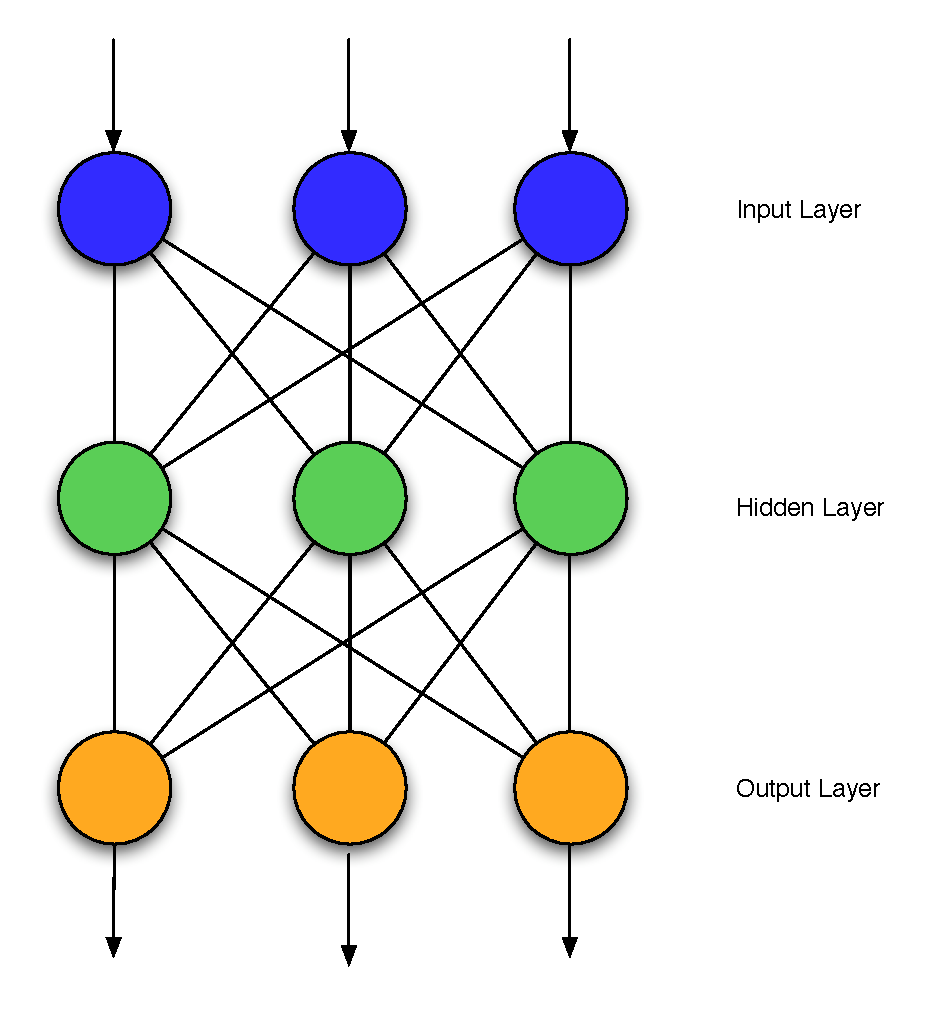
\includegraphics[width=80mm]{FeedForwardNetwork.eps}
     \caption{A feed forward network}
     \label{ASCA_AFFN}
     \end{figure}
     
     Connectionist models learn by adjusting the weights on the
     individual computational units. This implies that learning in
     connectionist models can be viewed more as a skill building
     exercise, rather than an exercise in knowledge acquistion as in
     the case of the congitivist approaches
     \cite{DBLP:journals/tec/VernonMS07}.
     
     The main attraction of connectionism is that it provides a means
     to provide neural plausibility\cite{103009} to theories of
     cognitive science because of its ability to simulate the
     massively parallel processing in the brain and also its ability
     to learn by adjusting weights. It is also attractive because it
     provides cognitive plausbility by allowing problems to be studied
     using simpler mechanisms, they could help in studying the
     processes underlying the processes of pattern-recognition and
     memory retrival and the ability to apply soft constraints when
     representing schematic knowledge.

     Despite these attractions connectionist models find it difficult
     to explain the ability of the human mind to to integrate diverse
     knowledge from various sources, the ability to use pre-existing
     knowledge and the ability to respond with in the time constraints
     that humans do.

     
\section{Cognitive Architectures}


\subsection{ACT-R}
\subsection{SOAR}
\subsection{EPIC}
\section{Challenges facing cognitive architectures}
